\subsection{Controllplatine}
\label{sec:control}
Als Steuerplatine kommt ein FRDM-KL25Z von Freescale zum Einsatz. 
Darauf wird wird ein FreeRTOS als Betriebssystem eingesetzt. 
Für die Ansteuerung der Peripherie und der externen Komponenten 
werden Komponenten mit Processor Expert erzeugt. 
\begin{figure}[h!]
    \centering
    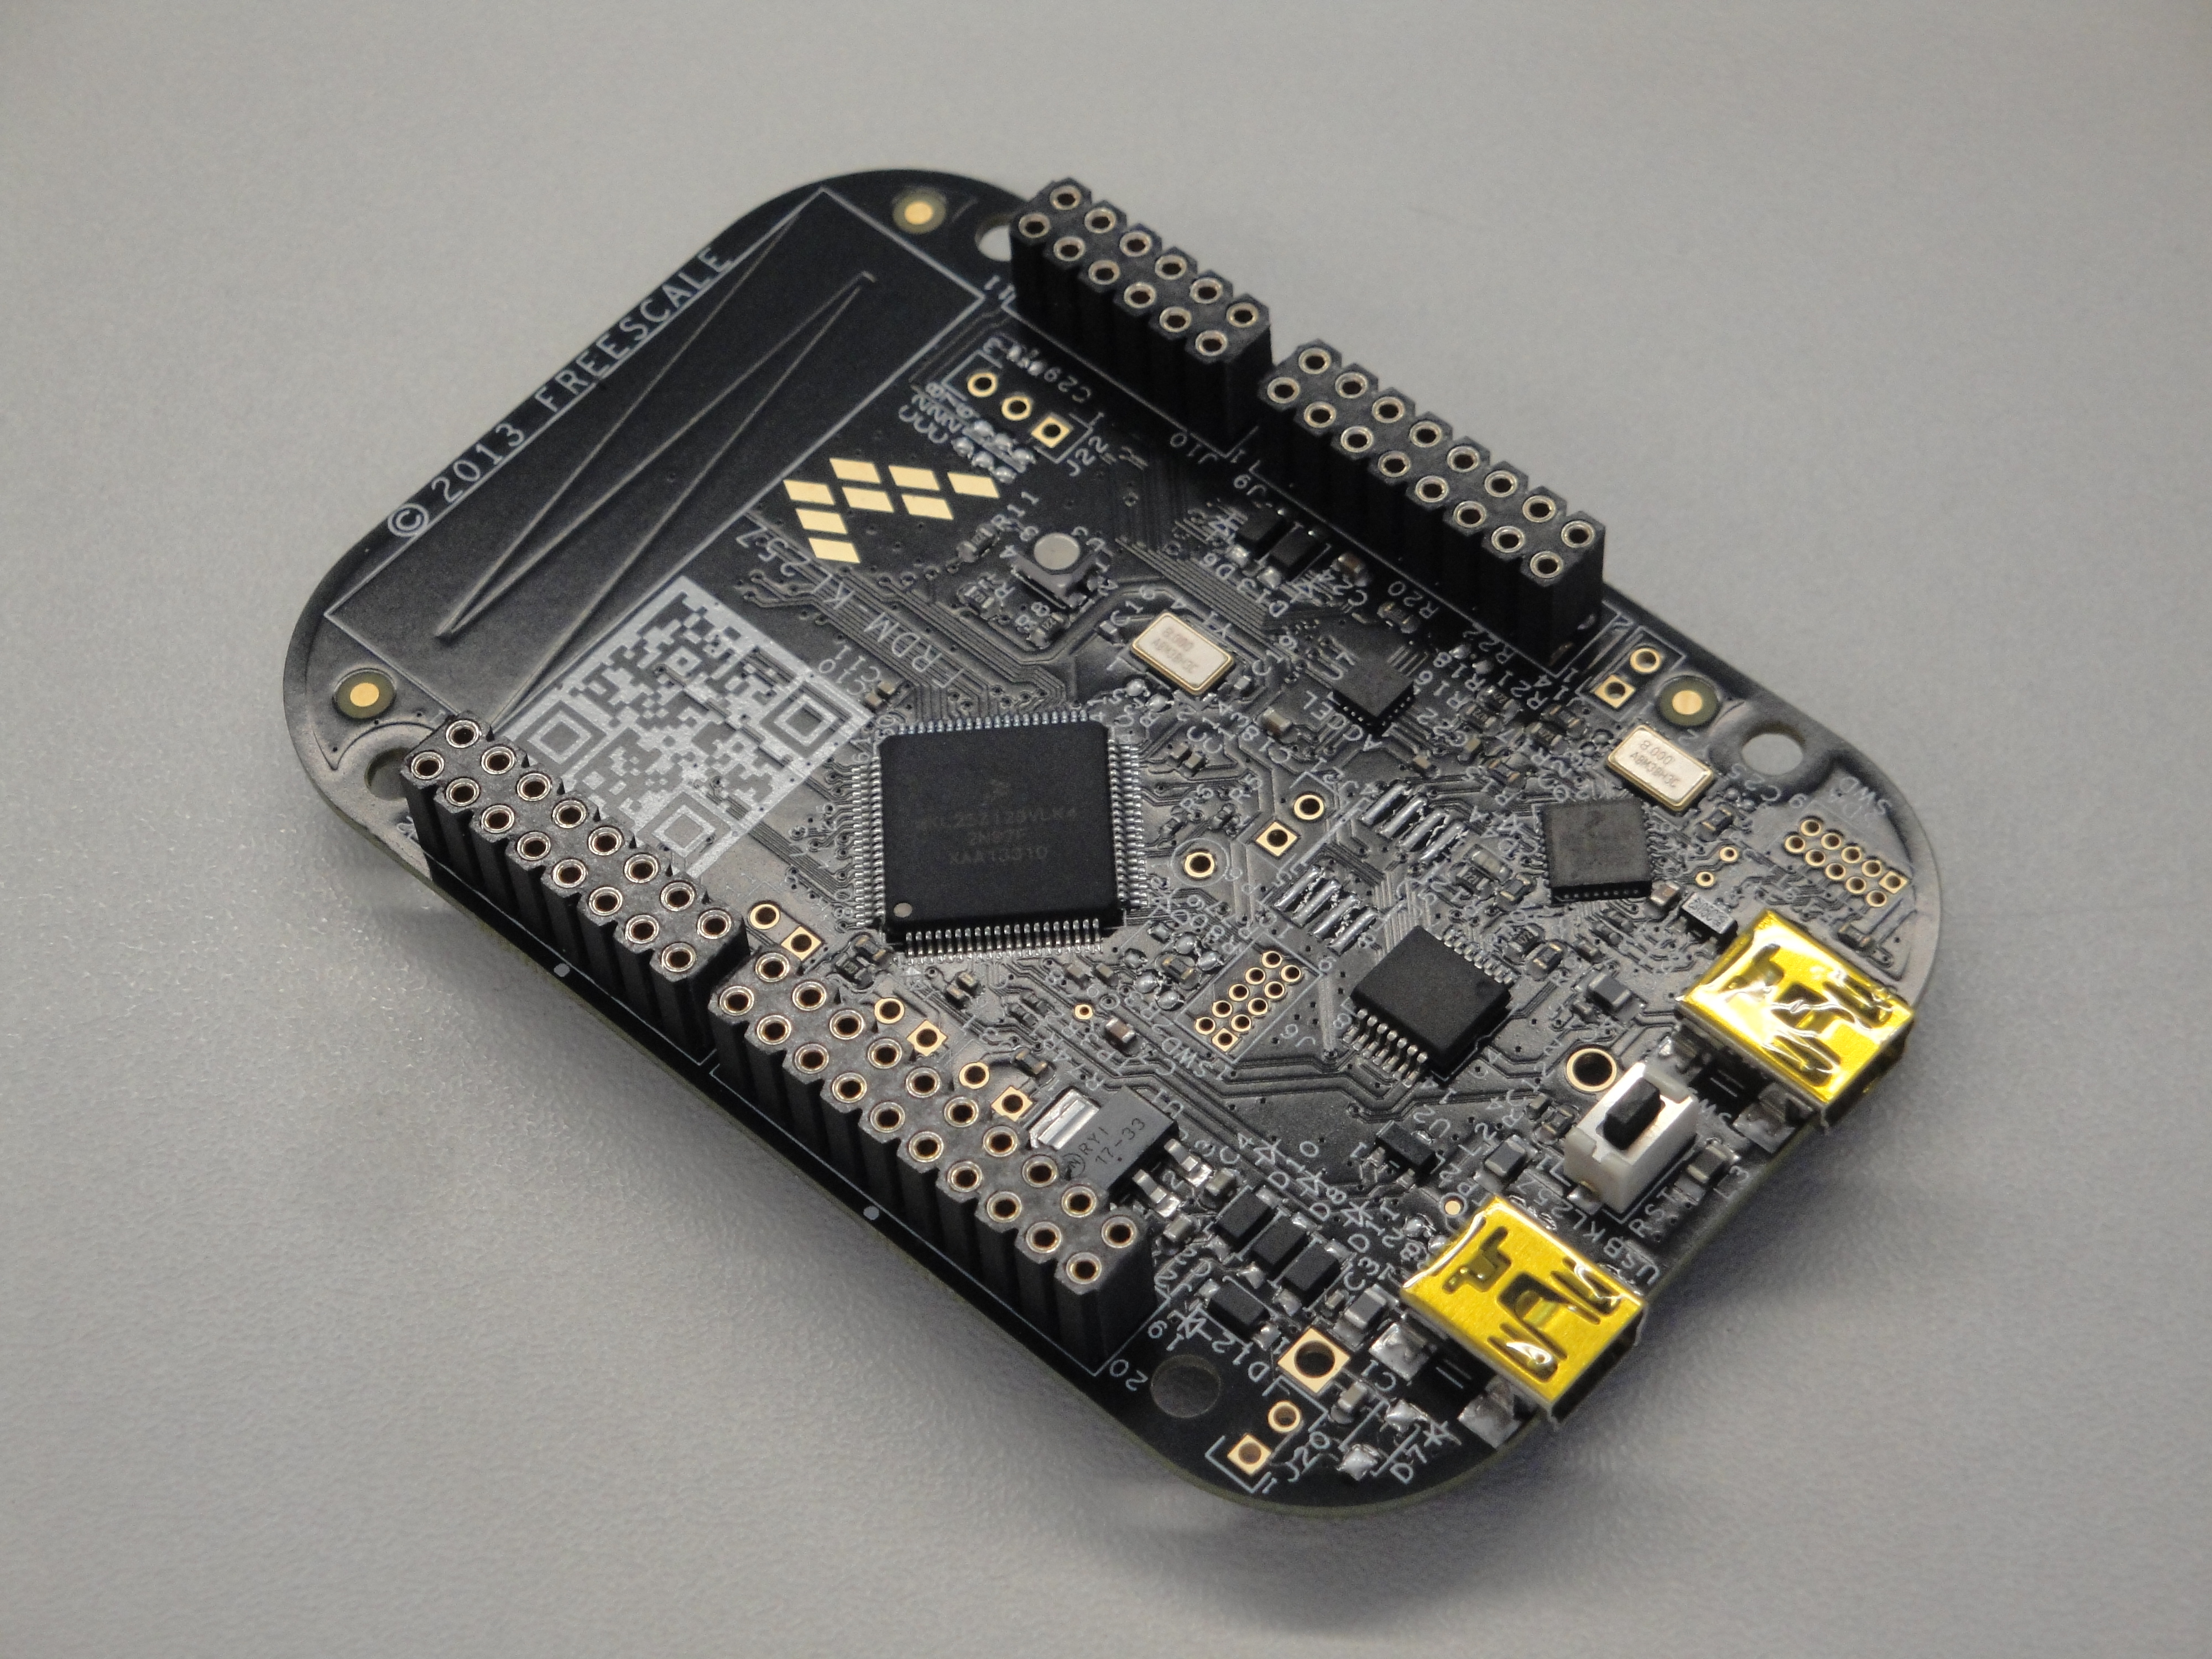
\includegraphics[width=0.45\textwidth]{fig_pcb/DSC02907.JPG}
    \caption{Kontrollplatine - FRDM-KL25Z}
    \label{fig:dc}
\end{figure}

\begin{table}[h!]
    \centering
    \begin{zebratabular}{p{0.21\textwidth}p{0.16\textwidth}p{0.5\textwidth}}
        \rowcolor{gray}
        Name                & Komponente        & Beschreibung \\
        FRTOS1              & FreeRTOS          & Echtzeit-Betriebssystem \\
        Cpu                 & MKL25Z128VLK4     & Controller \\
        UTIL1               & Utility           & Funktionen zur Verarbeitung von Zeichenketten \\
        WAIT1               & Wait              & Delays \\
        CS1                 & CriticalSection   & Deaktivieren von Interrupts für kritische Stellen im Code \\
        AS1                 & AsynchroSerial    & Serielle Schnittstelle via USB $\leftrightarrow$ UART Brücke \\
        TU1                 & TimerUnit\_LDD    & Timer für PWM \\
        TU2                 & TimerUnit\_LDD    & Timer für Timing Ballbeförderung\\
        LedRed              & LED               & Rote LED \\
        Ledgreen            & LED               & Grüne LED \\
        CLS1                & Shell             & Shell \\
        BT1                 & Bluetooth\_EGBT   & Bluetooth Modul \\
        BLDCspi             & SynchroMaster     & SPI zu BLDC Ansteuerung \\
        CS\_BLDC            & BitIO             & Chip Select für BLDC Ansteuerung \\
        BLDC1\_IRQ          & ExtInt            & Interrupt Pin für BLDC Ansteuerung \\
        Stepperspi          & SynchroMaster     & SPI zu Schrittmotor Ansteuerung \\
        STP\_BSY            & ExtInt            & Interrupt für das Signal Busy der Schrittmotor Ansteuerung \\
        PWM1                & PWM               & PWM für DC Motor \\
        DIR                 & BitIO             & Drehrichtung für DC Motor \\
        ENDSW\_SHOOT\_IRQ   & ExtInt            & Interrupt für optionalen oberen Endschalter \\
        ENDSW\_LOAD\_IRQ    & ExtInt            & Interrupt für optionalen unteren Endschalter \\
        HF1                 & HardFault         & Komponente um schwerwiegende Systemfehler debuggen zu können \\
        TI1                 & TimerInt          & Interrupt für Timing Ballbeförderung \\
    \end{zebratabular}
    \caption{Komponenten für das FRDM-KL25Z}
    \label{tab:comp_frdm}
\end{table}
